\chapter{Planificació}

En aquest capítol es mostra la planificació realitzada per a portar a terme el projecte. \\

Pel què fa a la definició d'objectius del nostre rootkit es poden veure en el capítol
funcionalitats \ref{cap:funcionalitats} on són explicats i justificats. \\

En aquesta planificació varem intentar no deixar la documentació del projecte pel final, 
sinó que fos un punt que s'anés avançant constantment. Varem separar les diferents tasques entre: el disseny
i la recerca inicial, la implementació de les funcionalitats (dividides en dos blocs segons la seva dificultat),
una part del rootkit a nivell de kernel per a GNU/Linux, i finalment un anàlisis general per a polir-ho
i homogeneïtzar-ho tot. \\

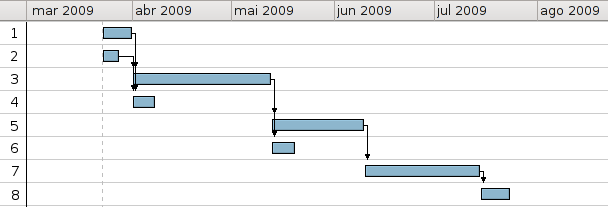
\includegraphics[scale=0.75,keepaspectratio]{primer_gantt2.png} 
\\
Les tasques que es poden veure en el gantt anterior juntament amb la seva durada són:

\begin{itemize}
    \item Estructura i disseny del rootkit (7 dies) 
    \item Estructura de la documentació (5 dies)
    \item Implementació de les funcionalitats bàsiques (30 dies) \\
		Les funcionalitats a implemantar en aquesta tasca són:
		\begin{itemize}
			\item Executable ELF estàtic
			\item Multiplataforma i multiarquitectura
			\item Connexió directa
			\item Obtenció d'una shell i un TTY
			\item Mode comanda / Mode servei
			\item Transferència de fitxers 
		\end{itemize}
    \item Documentació de les funcionalitats bàsiques (5 dies)
    \item Implementació de les funcionalitats avançades (25 dies) \\
		Les funcionalitats a implementar en aquesta tasca són:
		\begin{itemize}
			\item Comunicació xifrada
			\item Autenticació per contrasenya
			\item Detecció del rootkit
			\item Proteccions de l'executable
			\item Supervivència del rootkit
			\item Tasques programades
			\item Ocultació
			\item Heartbeat
			\item Independència de la shell
			\item Connexió inversa 
			\item Keylogger
		\end{itemize}
    \item Documentació de les funcionalitats avançades (5 dies)
    \item Injecció de codi en memòria de kernel (25 dies)
    \item Anàlisi general (7 dies) 
\end{itemize}
En total, la durada que s'ha calculat en aquesta planificació va del 23 de Març fins al 27 de Juliol. \\
